\section{Autoencoder Non-linear Manifold PROMs}

As proposed by Lee and Carlberg~\cite{Lee2020}, non-linear manifold PROMs have the potential to more accurately represent flows characterized by a slowly-decaying Kolmogorov $n$-width. The theoretical ability of neural networks to approximate arbitrary non-linear functions and the expressiveness of over-parameterized deep neural networks make them appealing candidates for the representation of a non-linear manifold on which to compute PROMs. As outlined in Section~\ref{subsec:nonlinManifold}, the autoencoder architecture allows for unsupervised learning of such a mapping directly from flow field data.

Autoencoders are trained using the same datasets described in Table~\ref{tab:trainSplit}, though the validation training datasets are used to evaluate the model's performance during training (without participating in actual gradient descent process). The encoder is composed of three convolutional layers, each with a kernel size of 8, a stride size of 2, and same zero padding. These are followed by a fully-connected (``dense'') layer which maps the encoder output to the latent dimension $\numPrimModes$. The output size (i.e., the number of filters) for the convolutional layers is summarized in Table.~\ref{tab:caeArch}. The decoder mirrors the encoder via transpose convolutional layers. All layers are equipped with the Swish activation function, except for the final decoder output layer, which uses a linear activation. Network weights are initialized with the Glorot (or Xavier) uniform distribution, and biases are initialized to zero.

\begin{table}
	\centering
	\begin{tabular}{ lll }
	\toprule
	Layer & Type & Output Size  \\
	\midrule
	1 & Convolution & 512 $\times$ 16 \\
    2 & Convolution & 256 $\times$ 32 \\
    3 & Convolution & 128 $\times$ 64 \\
    4 & Dense & $\numPrimModes$ \\
	\bottomrule
	\end{tabular}
	\caption{\label{tab:caeArch}Convolutional encoder dimensions. Decoder mirrors encoder with transpose convolutional layers.}
\end{table}

Each network is trained for a maximum of 5,000 epochs, with a batch size of 25 and the mean-squared error loss function. The Adam optimizer with a learning rate of $1\times10^{-4}$ is utilized, and early stopping halts training if the validation loss does not improve over 500 epochs. All network construction, training, and evaluation is computed using the TensorFlow library.

\begin{figure}
    \begin{minipage}{0.49\linewidth}
        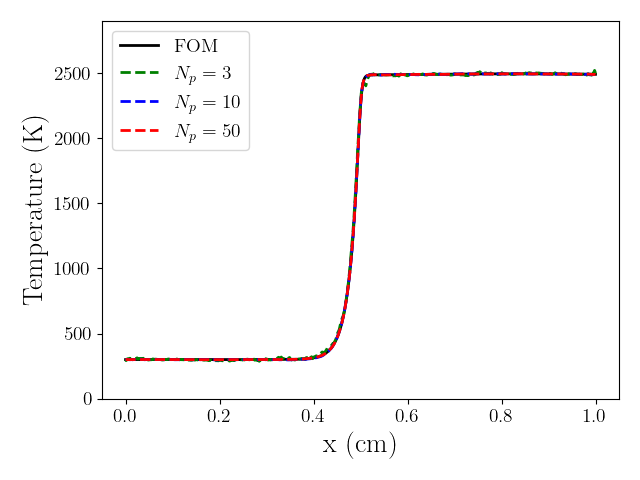
\includegraphics[width=0.99\linewidth]{Chapters/TransientFlame/Images/nonlinear/proj_temp_snaps.png}
    \end{minipage}
    \begin{minipage}{0.49\linewidth}
        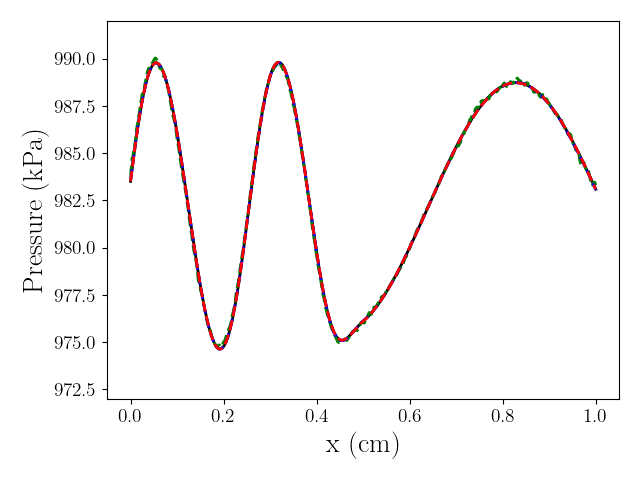
\includegraphics[width=0.99\linewidth]{Chapters/TransientFlame/Images/nonlinear/proj_press_snaps.png}
    \end{minipage}
    \caption{\label{fig:flameNonlinProj}Approximation of temperature (left) and pressure (right) fields on solution manifold, $f = 150$ kHz, $\timeVar = 250 \mu$s, various $\numPrimModes$.}
\end{figure}

The resulting autoencoders display exceptional accuracy in approximating the flame flow fields. Figure~\ref{fig:flameNonlinProj} shows the closest solution on the trial manifold (in the Euclidean norm) for temperature and pressure field snapshots. Even for $\numPrimModes = 3$, the representation is nearly perfect. Very close inspection reveals some low-amplitude noise, but larger latent space dimensions appear to entirely eliminate this. At first glance, this would appear to bode well for the resulting non-linear manifold PROMs.

\begin{figure}
    \begin{minipage}{0.49\linewidth}
        \includegraphics[width=0.99\linewidth]{example-image-a}
    \end{minipage}
    \begin{minipage}{0.49\linewidth}
        \includegraphics[width=0.99\linewidth]{example-image-a}
    \end{minipage}
    \caption{\label{fig:flameNonlinROM}Intrusive non-linear manifold MP-LSVT PROM snapshots, $\timeVar = XXX$, various $\numPrimModes$.}
\end{figure}

The same simulation configuration used for the linear subspace MP-LSVT PROMs is repeated here. Unfortunately, the autoencoder non-linear manifold PROMs also perform very poorly. In contrast to the over-smooth solutions generated by the linear trial spaces, the non-linear manifold PROMs suffer from excessive low-amplitude noise in the predicted solution. This is made apparent in Fig.~\ref{fig:flameNonlinROM}, revealing that the solution quickly devolves into meaningless noise where the approximate solution shown in Fig.~\ref{fig:flameNonlinProj} was so accurate. Ultimately, these non-linear PROMs suffer from an accumulation of error over a large number of time steps. These small errors appear to be amplified by the non-linear nature of the decoder: small deviations in the latent variables may lead to drastic changes in the predicted solution. Whereas linear trial space are relatively limited in their expressiveness, neural networks have the ability to generate both very accurate and very wrong solutions.

\begin{table}
	\centering
	\begin{tabular}{ lll }
	\toprule
	Model & Runtime (hours) & Cost (FOM runs)  \\
	\midrule
    Online FOM ($\times 1$) & 0.42 & 1 \\
    Training, $\numPrimModes = 3$ & 5.8 & 13.81 \\
    Training, $\numPrimModes = 10$ & 4.9 & 11.67 \\
    Training, $\numPrimModes = 50$ & 5.5 & 13.1 \\
    Online NLM PROM, $\numPrimModes = 3$ & 7.2 & 17.14 \\
	\bottomrule
	\end{tabular}
	\caption{\label{tab:caeCost}Relative offline/online computational costs for CAE PROMs. Non-increasing CAE training costs are due to early stopping.}
\end{table}

Not only is the accuracy of these non-linear manifolds PROMs disappointing, the cost to train and evaluate these models is exorbitant. Table~\ref{tab:caeCost} summarizes the cost of training and computing the neural network models, revealing that each step accounts for over ten times that of a single FOM simulation. The vast majority of the computational cost for the non-linear manifold PROM lies in calculating the Jacobian of the decoder, which relies on slow automatic differentiation procedures. Opposed to the simple analytical Jacobians possible for linear representations, it is difficult to justify the cost of this method given its experimental performance.

\section{Recurrent Neural Network ROMs}

\begin{figure}
    \centering
    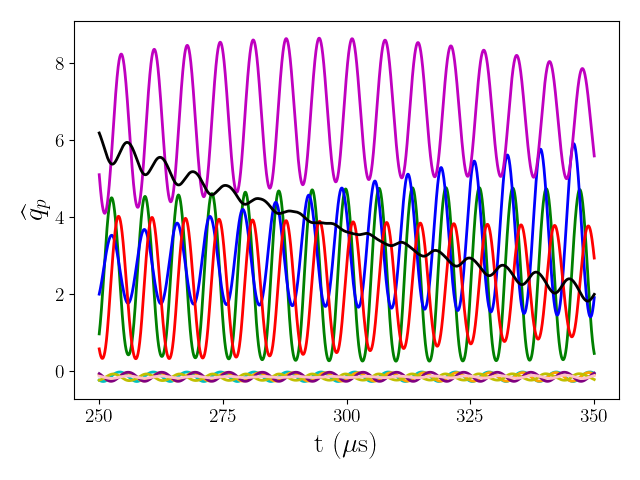
\includegraphics[width=0.6\linewidth]{Chapters/TransientFlame/Images/nonlinear/latent_vars.png}
    \caption{Encoded latent state trajectories, $f = 150$ kHz, $\numPrimModes = 10$.}
\end{figure}

\begin{figure}
    \begin{minipage}{0.49\linewidth}
        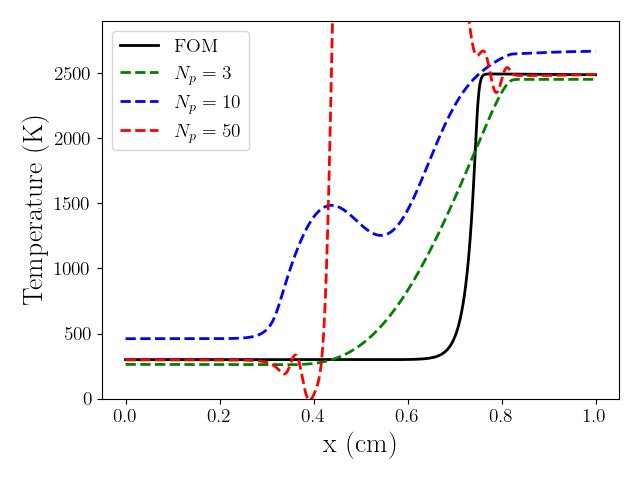
\includegraphics[width=0.99\linewidth]{Chapters/TransientFlame/Images/lstm/pod_rom_temp_snaps.png}
    \end{minipage}
    \begin{minipage}{0.49\linewidth}
        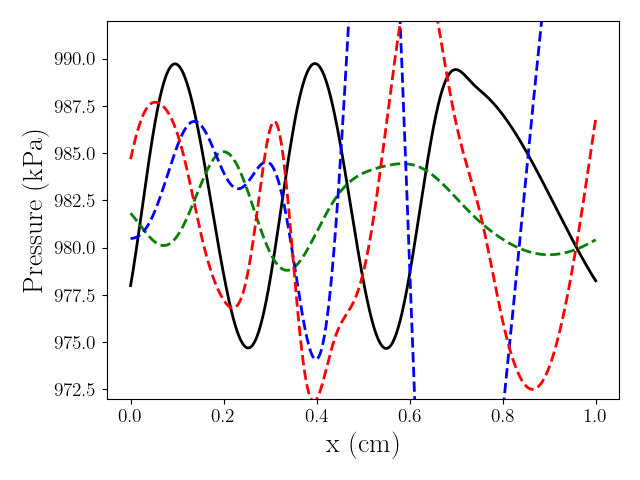
\includegraphics[width=0.99\linewidth]{Chapters/TransientFlame/Images/lstm/pod_rom_press_snaps.png}
    \end{minipage}
    \caption{Online temperature (left) and pressure (right) field predictions for LSTMs trained with POD trajectories, $\timeVar = 500 \mu$s, $f = 131.25$ kHz, various $\numPrimModes$.}
\end{figure}

\begin{figure}
    \begin{minipage}{0.49\linewidth}
        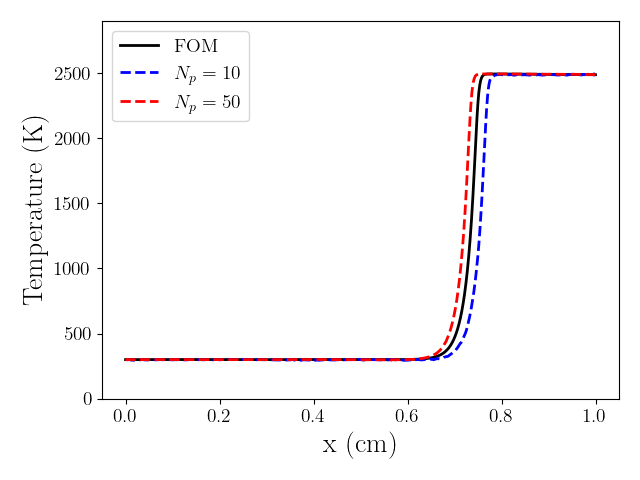
\includegraphics[width=0.99\linewidth]{Chapters/TransientFlame/Images/lstm/cae_rom_temp_snaps.png}
    \end{minipage}
    \begin{minipage}{0.49\linewidth}
        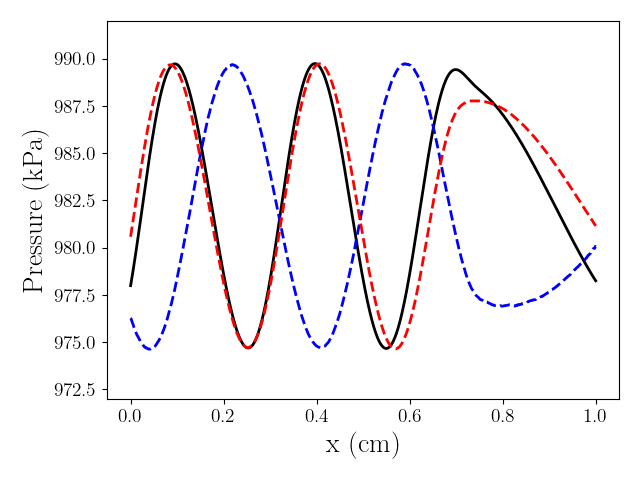
\includegraphics[width=0.99\linewidth]{Chapters/TransientFlame/Images/lstm/cae_rom_press_snaps.png}
    \end{minipage}
    \caption{Online temperature (left) and pressure (right) field predictions for LSTMs trained with CAE trajectories, $\timeVar = 500 \mu$s, $f = 131.25$ kHz, various $\numPrimModes$. Note that $\numPrimModes = 3$ was unstable.}
\end{figure}

\begin{figure}
    \begin{minipage}{0.49\linewidth}
        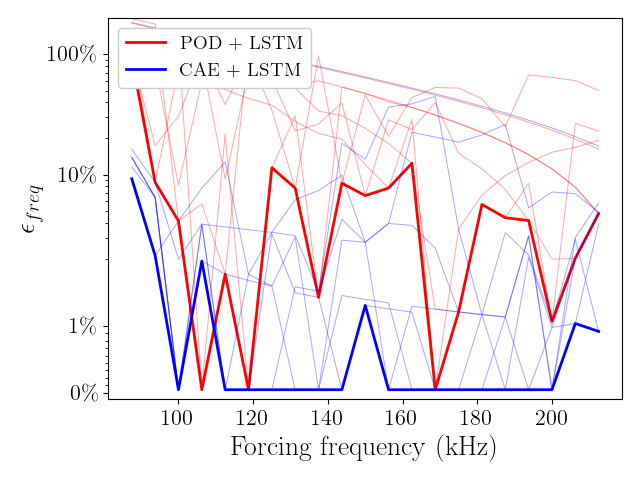
\includegraphics[width=0.99\linewidth]{Chapters/TransientFlame/Images/lstm/freq_err.png}
        \subcaption{Upstream $f$.}
    \end{minipage}
    \begin{minipage}{0.49\linewidth}
        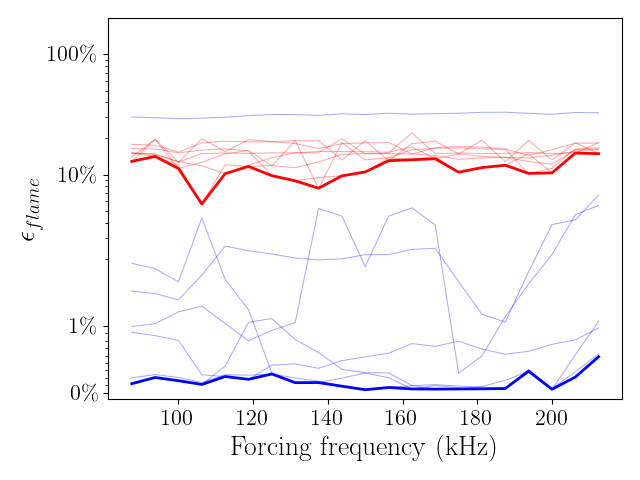
\includegraphics[width=0.99\linewidth]{Chapters/TransientFlame/Images/lstm/err_flame.png}
        \subcaption{Flame speed}
    \end{minipage}
    \caption{Aggregate predictions of QoIs across all forcing frequencies, all $\numPrimModes$. The best predictions for each model are marked by a bold line.}
\end{figure}